\documentclass{msuposter}
\usepackage{lipsum}
\usepackage{multirow}
\usepackage{tikz,wrapfig}
\usepackage{tikz}
\usetikzlibrary{decorations.pathreplacing}
\usetikzlibrary{arrows}
\newcommand{\mR}{\mathbb{R}}
\newcommand{\mN}{\mathbb{N}}
\newcommand{\cT}{\mathcal{T}}
\newcommand{\uh}{u_h}
\newcommand{\qh}{q_h}
\newcommand{\ph}{p_h}
\newcommand{\qhat}{\hat{q}}
\newcommand{\uhat}{\hat{u}}
\newcommand{\cB}{\mathcal{B}}
\newcommand{\cL}{\mathcal{L}}
\newcommand{\cO}{\mathcal{O}}
\newcommand{\euhat}{\hat{e}_{\uh}}
\newcommand{\eqhat}{\hat{e}_{\qh}}
\newcommand{\cP}{\mathcal{P}}
\newcommand{\projh}{\mathcal{S}}
\newcommand{\eu}{e_u}
\newcommand{\ep}{e_p}
\newcommand{\eq}{e_q}
\newcommand{\xiu}{\xi_u}
\newcommand{\xip}{\xi_p}
\newcommand{\xiq}{\xi_q}
\newcommand{\xiuhat}{\hat{\xi}_u}
\newcommand{\xiqhat}{\hat{\xi}_q}
%\theoremstyle{definition}
%\newtheorem{definition}{Definition}[section]
%\newtheorem{example}{Example}[section]
%\theoremstyle{plain}
%\newtheorem{theorem}{Theorem}[section]
%\newtheorem{corollary}{Corollary}[theorem]
%\newtheorem{lemma}[theorem]{Lemma}
%\newtheorem{proposition}[theorem]{Proposition}
\title{Local discontinuous Galerkin methods with novel basis for fractional diffusion equations with non-smooth solutions}
\author{\href{http://lylyu.com/}{\textbf{Liyao Lyu}} $^a$,Zheng Chen$^b$}
\institute{
$^a$Department of Computational Mathematics, Science and Engineering, Michigan State University,
lyuliyao@msu.edu\\
$^b$Department of Mathematics, University of Massachusetts Dartmouth, zchen2@umassd.edu
}

\newcommand{\colwidth}{0.3\linewidth}

\begin{document}
\begin{frame}{}
\begin{columns}[t]
\begin{column}{\colwidth}
\begin{block}{Abstract}
In this paper, we develop a \textbf{novel local discontinuous Galerkin (LDG) methods} for \textbf{fractional diffusion equations} with \textbf{non-smooth solutions}.  
We consider such problems, for which the solutions are not smooth at boundary, and therefore the traditional LDG methods with piecewise polynomial solutions suffer accuracy degeneracy.  The novel LDG methods utilize a solution information enriched basis, and simulate the problem on a paired special mesh, and \textbf{achieve optimal order of accuracy}. We analyze the $L^2$-stability and optimal error estimate in $L^2$-norm.  
Finally, numerical examples are presented for validating the theoretical conclusions.
\end{block}
\begin{block}{Introduction}
Consider the equations in the form
\begin{equation}\label{eqn:problem}
\frac{\partial u(x,t)}{\partial t} = d \frac{\partial^{\beta} u(x,t)}{\partial x^\beta} + f(x,t), \quad x\in[a,b],\quad \beta\in(1,2),\quad  d>0
\end{equation}
The fractional derivative here is a Caputo derivative
\begin{equation}\label{eqn:def_cd}
{}_a^{C}D_{x}^{\alpha} v(x)=\frac{1}{\Gamma(n-\alpha)} \int_{a}^{x}(x-\xi)^{n-\alpha-1} \frac{d^{n} v(\xi)}{\mathrm{d} \xi^{n}} \mathrm{d} \xi, \quad x>a, \quad \alpha \in[n-1, n)
\end{equation}
The equation \eqref{eqn:problem} can be rewritten into the following system
\begin{equation}\label{local DG}
\begin{aligned}
&\frac{\partial u(x,t)}{\partial t} - \sqrt{d} \frac{\partial q(x,t)}{\partial x} = f(x,t) & \text{in }\Omega_T,\\
& q-_{a}D_{x}^{\beta-2} p(x,t) =0 & \text{in }\Omega_T,\\
& p- \sqrt{d}\frac{\partial u(x,t)}{\partial x}=0& \text{in }\Omega_T,
\end{aligned}
\end{equation}
Local discontinuous Galerkin methods with regular basis achieve optimal order of accuracy both theoretically and computationally for \textbf{smooth enough underlying solutions}.

\textbf{However, the order $\downarrow$ is observed when applied to problems with non-smooth solutions.} Consider solving a non-smooth problem with a solution $u(\cdot\, ,t)\in H^\alpha$, the LDG method using finite element space $V^k$, will achieve an error with a theoretical order $\min\{k+1,\alpha\}$, and the numerical order is observed to be like $\min\{k+1,\alpha+0.5\}$

\end{block}
\begin{block}{Novel approximation space and mesh}
	Consider that the solution to problem \eqref{eqn:problem} has an weak singularity at the left end of the domain, and is of form 
	\begin{equation}
	\label{func:solution form}
	w(x) (x-a)^\beta
	\end{equation} 
	with some unknown but smooth function $w(x)$.
In the domain near starting point, the exact solution is considered as a function of the mapped variable $y = (x-a)^{\gamma}$, is a regular function, with $\frac{1}{\gamma}$ being the smallest positive integer makes $\frac{\beta}{\gamma} \in \mathbb{N}$. 
Therefore,  finite element space $V^k_{\gamma}$for both trial functions and test functions: 
\begin{equation}\label{eqn:functional basis}
V^k_{\gamma} = \left\{v: v\bigr\rvert_{I_j} \in P^k((x-a)^{\gamma}), \text{ if } x_j \leq \hat{x};  \, v \bigr\rvert_{I_j}\in P^{k}(x), \text{ otherwise} \right\}.
\end{equation}
In order to deal with ill-conditioned mass matrix, we adopted graded mesh for the cells with irregular mesh.
\begin{equation}\label{grid:part1}
\begin{aligned}
&x_j = a + \left(\frac{b-a}{N} j \right)^{{1/\gamma}} & \quad  &\text{for }  j \leq n,\\
&x_j = b - (M-j)\frac{b-a}{N} & \quad & \text{for } n < j \leq M,
\end{aligned}
\end{equation}

\centering{
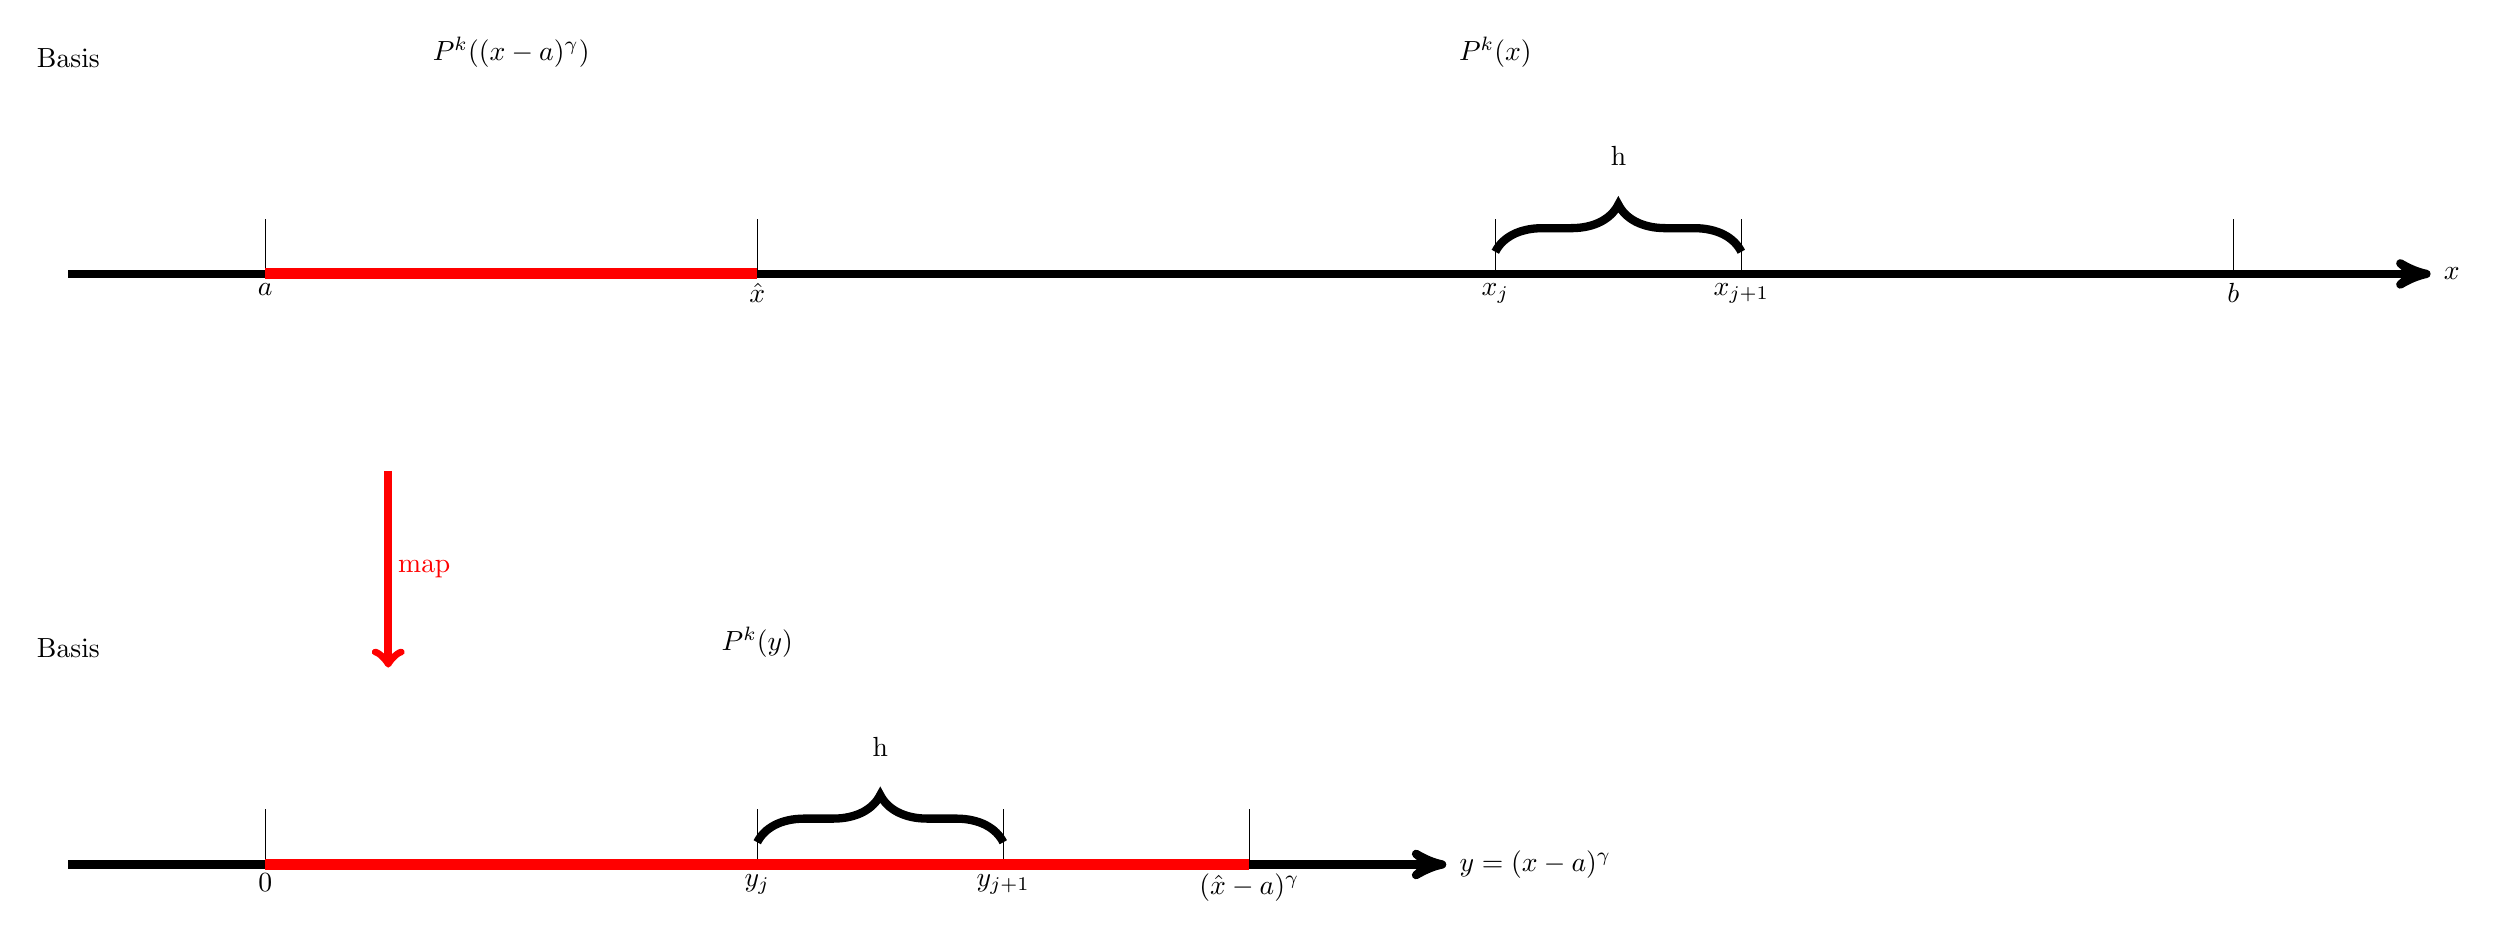
\begin{tikzpicture}[
    scale=25,
    axis/.style={very thick, ->, >=stealth'},
    important line/.style={thick},
    dashed line/.style={dashed, thin},
    pile/.style={thick, ->, >=stealth', shorten <=2pt, shorten
    >=2pt},
    every node/.style={color=black}
    ]
%画x和y轴坐标
\draw[axis,line width=3pt] (-0.1,0)  -> (1.1,0) node(xline)[right]
        {$x$};
\draw[axis,line width=3pt] (-0.1,-0.3)  -> (0.6,-0.3) node(xline)[right]
        {$y = (x-a)^\gamma$};
\coordinate (label1) at(-0.1,0.1);
\coordinate (label2) at(-0.1,-0.2);
\coordinate (a) at (0,0);%画刻度
\coordinate (x) at (1/4,0);%画刻度
\coordinate (xj) at (5/8,0);%画刻度
\coordinate (xj1) at (6/8,0);%画刻度
\coordinate (yj) at (2/8,-0.3);%画刻度
\coordinate (yj1) at (3/8,-0.3);%画刻度
\coordinate (ba1) at (1/8,0.1);
\coordinate (ba2) at (5/8,0.1);
\coordinate (b) at (1,0);
\coordinate (y0) at (0,-0.3);
\coordinate (hy) at (0.5,-0.3);
\draw (label1) node[above] {Basis};
\draw (label2) node[above] {Basis};
\draw (a) node[below] {$a$} -- ++(0, 0.8 pt) ; 
\draw (x) node[below] {$\hat{x}$} -- ++(0, 0.8 pt) ;
\draw (ba1) node[above] {$P^k((x-a)^\gamma)$};
\draw (xj) node[below] {$x_j$} -- ++(0, 0.8 pt) ; 
\draw (xj1) node[below] {$x_{j+1}$} -- ++(0, 0.8 pt) ;
\draw (yj) node[below] {$y_j$} -- ++(0, 0.8 pt) ; 
\draw (yj1) node[below] {$y_{j+1}$} -- ++(0, 0.8 pt) ;
\draw[decorate,decoration={brace,raise=8pt,amplitude=6mm},line width=3pt] (xj) -- (xj1);
\draw[decorate,decoration={brace,raise=8pt,amplitude=6mm},line width=3pt] (yj) -- (yj1);
\draw (b) node[below] {$b$} -- ++(0, 0.8 pt) ;
\draw node[above] at (1/4,-0.2) {$P^k(y)$};
\draw (ba2) node[above] {$P^k(x)$};
\draw (y0) node[below] {$0$} -- ++(0, 0.8 pt) ; 
\draw (hy) node[below] {$(\hat{x}-a)^\gamma$} -- ++(0, 0.8 pt) ; 
\draw[->,line width = 3 pt,red] (1/16,-0.1)  -- (1/16,-0.2);
\draw[line width =  4 pt, red] (0,0) -- (1/4,0);
\draw[line width =  4 pt, red] (y0) -- (hy);
\draw node[above] at (11/16,0.05) {h};
\draw node[above] at (5/16,-0.25) {h};
\draw node[right,red] at (1/16,-0.15) {map};
\end{tikzpicture}
}



\end{block}

\end{column}



\begin{column}{\colwidth}
\begin{exampleblock}{Numerical test when $\gamma = 0.5$}
	Consider equation 
	\begin{equation}\label{eqn:exm1}
	\begin{aligned}
	\frac{\partial u(x,t)}{\partial t} = \frac{2 }{3\Gamma(1.5)} \frac{\partial ^{1.5} u(x,t)}{\partial x^{1.5}} - e^{-t} (x^{1.5} +1),\quad x \in (0,1),
	\end{aligned}
	\end{equation}
 on the computational domain $x\in \Omega =(0,1)$ with initial condition$u_0(x) = x^{1.5}$
	and Dirichlet boundary conditions. The exact solution is $u(x,t) = e^{-t}x^{1.5}$. 

\begin{figure}
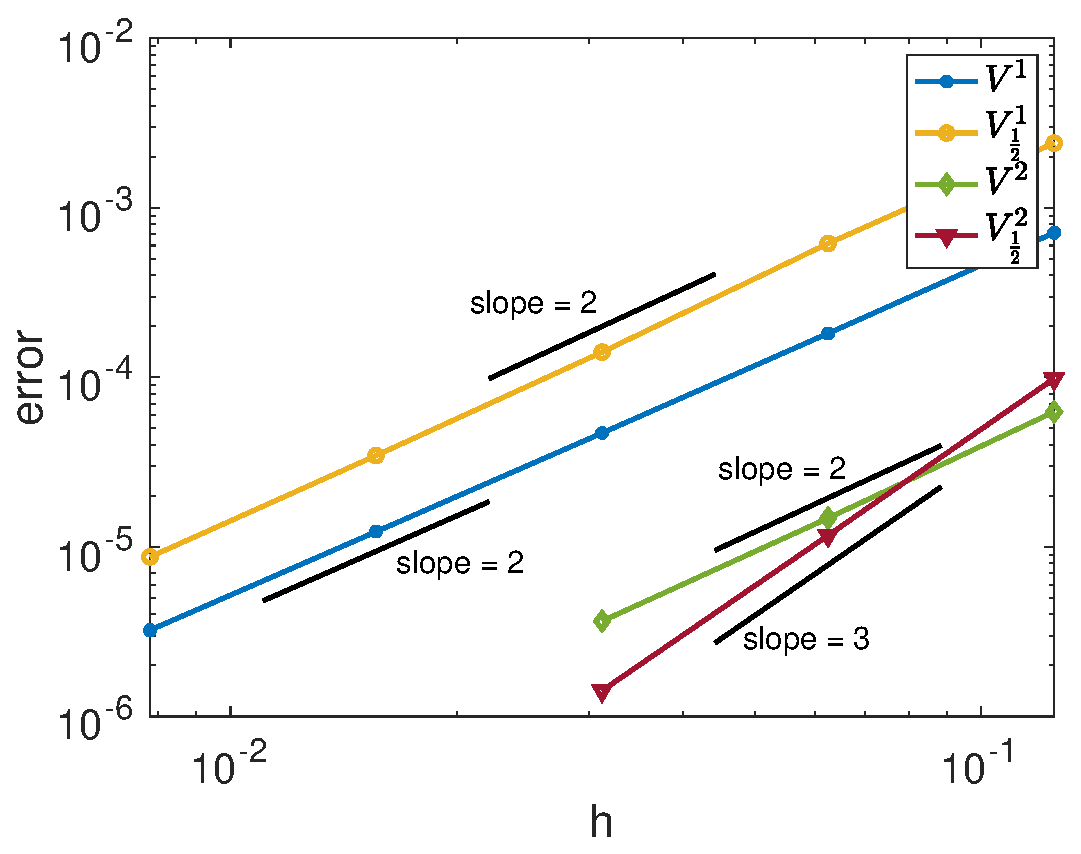
\includegraphics[width=0.8\linewidth]{Figure1}
\end{figure}
\end{exampleblock}
\begin{block}{Semi-defined LDG scheme} 
The semi-discrete LDG scheme to solve systemx is defined as follows. 
Find $\uh, \qh, \ph \in V^k_\gamma$ such that, for all test functions $v, w, z \in V^k_\gamma$ and all $j=1,2,\dots,M$, we have
\begin{equation*}\label{eqn:Numerical Scheme}
\begin{aligned}
\left(\frac{\partial \uh(x,t)}{\partial t},\,v(x) \right)_{I_j} +\sqrt{d}\left(\qh(x,t),\,\frac{\partial v(x)}{\partial x}\right)_{I_j} - \sqrt{d}\qhat(x,t) v(x)\Bigr\rvert_{x_{j-1}^+}^{x_j^-}&=(f(x,t),\,v(x))_{I_j},\\
\left( \qh(x,t),\,w(x)\right)_{I_j} - (_{a}D_x^{\beta-2}\ph(x,t),\,w(x))_{I_j}&=0, \\
\left(\ph(x,t),\,z(x)\right)_{I_j} +\sqrt{d}\left(\uh(x,t),\,\frac{\partial z(x)}{\partial x}\right)_{I_j} -\sqrt{d} \uhat(x,t)z(x)\Bigr\rvert_{x_{j-1}^+}^{x_j^-}&=0,
\end{aligned}
\end{equation*}
\end{block}
\begin{block}{Alternating fluxes}
Here, we use the so-called ``alternating fluxes", which is a popular and attractive choice and defined as
\begin{equation}\label{eqn:Numerical Flux1 inner}
\begin{aligned}
\qhat(x_j,t)&=\qh^+(x_j,t), & \uhat(x_j,t)&=\uh^-(x_j,t); \\
\end{aligned}
\end{equation}
or
\begin{equation}\label{eqn:Numerical Flux2 inner}
\begin{aligned}
\qhat(x_j,t)&=\qh^-(x_j,t), & \uhat(x_j,t)&=\uh^+(x_j,t) \\
\end{aligned}
\end{equation}
at any interior cell interfaces; 
at the domain boundaries, 
\begin{equation}\label{eqn:Numerical Flux \uh BC}
\begin{aligned}
\uhat(a,t)&=0, & \uhat(b,t)&=g(t),  \\
\end{aligned}
\end{equation}
and
\begin{equation}\label{eqn:Numerical Flux \qh BC}
\begin{aligned}
\qhat(a,t)&=\qh^+(a,t), & \qhat(b,t)&=\qh^-(b,t), \\
\end{aligned}
\end{equation}
which reflect the Dirichlet boundary conditions. 
\end{block}
\begin{theorem}[$L^2$ stability]
	The scheme \eqref{eqn:Numerical Scheme} is $L^2$ stable, and the solutions satisfies, for all $t\in [0,T]$, 
	
	\begin{equation}\label{eqn:Stability theorem}
	\begin{aligned}
	\|e_{\uh}(\cdot,t)\|_{L^2}^2 
	+  2\cos ((\beta/2-1)\pi)\int_{0}^{t} \, \|_{a}D_{x}^{\beta/2-1}e_{\ph}(\cdot,t)\|_{L^2}^2 \, dt
	= \|e_{\uh}(\cdot,0)\|_{L^2}^2. 
	\end{aligned}
	\end{equation}
\end{theorem}
\end{column}



\begin{column}{\colwidth}
\begin{exampleblock}{Numerical test when $\gamma = 	\frac{1}{3}$}
Consider 
	\begin{equation}
	\begin{aligned}
	\frac{\partial u(x,t)}{\partial t} = \frac{9\sqrt{3}\Gamma(\frac{2}{3}) }{8\pi} \frac{\partial ^{\frac{4}{3}} u(x,t)}{\partial x^{\frac{4}{3}}} - e^{-t} (x^{\frac{4}{3}} +1)
	\end{aligned}
	\end{equation}
 on the computational domain $x\in \Omega =(0,1)$ with initial condition$u_0(x) = x^{\frac{4}{3}}$
	and Dirichlet boundary conditions. The exact solution is $u(x,t) = e^{-t}x^{\frac{4}{3}}$. 

	\begin{figure}
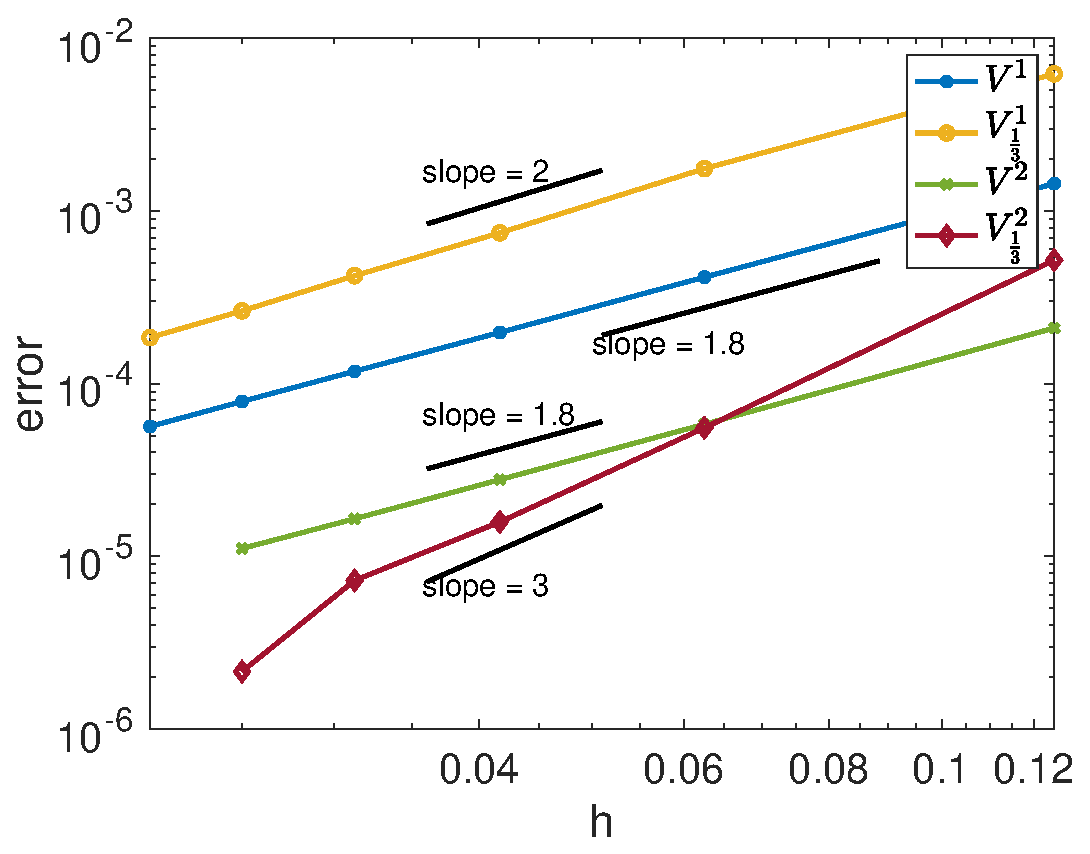
\includegraphics[width=0.8\linewidth]{Figure2}
\end{figure}
\end{exampleblock}
	
\begin{theorem}[Error Estimation]\label{thm:accuracy}
	The error for the scheme \eqref{eqn:Numerical Scheme} with flux \eqref{eqn:Numerical Flux1 inner} or \eqref{eqn:Numerical Flux2 inner} and \eqref{eqn:Numerical Flux \uh BC}-\eqref{eqn:Numerical Flux \qh BC} satisfies
	\begin{equation}\label{eqn:accuracy thm}
	\| u - \uh \|_{L^2}  \leq Ch^{k+1}.
	\end{equation}
\end{theorem}

\begin{block}{Conclusion}
We design a novel LDG method for spatial fractional diffusion equations with \textbf{weakly singular solutions} and obtain \textbf{optimal convergence rate}.
The key points are to build the singular information into finite element space, and modify the mesh with graded cells near the singularity to overcome the ill-condition mass matrix. 
Both stability and error estimation have been established. 
The global nature of the fractional operator makes computational cost really high, but the proposed approximation space gives optimal order of accuracy, and thus reduces the mesh size for same level of accuracy. 
However, the regularity of solution needs to be estimated ahead of time to choose a suitable approximation space.
In this paper, we deal with the cases with fractional order, that is $\beta  = \frac{p}{q}$ for some integers $p$ and $q$.  
In the future, we plan to extend the work to more general cases.   
The methodology has potential to be applied to other fractional differential equations or any PDEs with such singular solutions, and this is also part of our future work. 
\end{block}
\begin{block}{Reference}
Liyao Lyu, Zheng Chen. 2020. "Local discontinuous Galerkin methods with novel basis for fractional diffusion equations with non-smooth solutions."  Communications on Applied Mathematics and Computation.10.1007/s42967-020-00104-3
\end{block}
\end{column}
\end{columns}	
\end{frame}
\end{document}
